\section*{Введение}
Практическая работа посвящена оформлению математического текста с формулами и рисунками, а также оформлению таблицы с профессиями при помощи системы верстки LaTeX.

Цель работы: оформить 3 страницы математического текста и таблицу с профессиями согласно правилам оформления ГОСТ 7.32

\addcontentsline{toc}{section}{Введение}

\newpage
\section{Определение и необходимые условия экстремума функции нескольких переменных}
\textbf{Определение 1.1} Пусть функция
\[ f(x) = f(x_1,x_2,...,x_n) \]
определена в некоторой окрестности точки
\[  x_0 = (x_0^1,x_0^2,...,x_0^n). \]

Говорят, что функция $f(x)$ имеет в точке $x_0$ \textit{локальный максимум (минимум)}, если существует такая окрестность точки $x_0$, в которой для всех $x \neq x_0$ выполняется неравенство

\[f(x) \leq f(x0) (f(x) \geq f(x0)). \eqno(1.1)\]

Если для всех $x \neq x_0$ из некоторой окрестности точки $x_0$
выполняется строгое неравенство
\[f(x) < f(x0) (f(x) > f(x0)),\]
то $x_0$ называются \texit{точкой строгого максимума (минимума)} функции.

Точки максимума и минимума функции называются \textit{точками экстремума}, а значения функции в этих точках называется \texit{экстремумами функции}.

\textbf{Теорема 1.1} (необходимое условие экстремума). 
\textit{Если точка $(x^0_1, x^0_2, . . . , x^0_n)$ является точкой экстремума функции $f(x_1, x_2, . . . , x_n)$ и в этой точке существует частная производная $\frac{\partial f}{\partial x_i}(x_0),$ то она равна нулю.}

\textit{Доказательство.} Рассмотрим функцию одной переменной $x_i$:
\[g(x_i) = f(x^0_1,...,x^0_i−1,x_i,x^0_i+1,...,x^0_n).\]

Существование конечной частной производной функции
$f(x_1 , . . . , x_n )$ по переменной $xi_$ в точке $x_0$ эквивалентно
дифференцируемости функции $g(x_i)$ в точке $x^0_i$ . Очевидно,
что функцияg ($x_i$) имеет в точке $x^0_i$ локальный экстремум.
А тогда $g′(x^0_i ) = 0.$ Это означает, что $f'_x_i (x_0) = 0.$ Теорема доказана.

Если функция $f(x_1, x_2, . . . , x_n)$ имеет в точке $x_0$ локальный экстремум и дифференцируема в этой точке, то частные производные по всем переменным в этой точке равны нулю:
\[\frac{\partial f}{\partial x_1} = 0, \frac{\partial f}{\partial x_2} = 0, . . . \frac{\partial f}{\partial x_n} = 0 \eqno(1.2)\]
а следовательно,
\[df(x^0_1, x^0_2, . . . , x^0_n = 0. \]
Точки, координаты которых удовлетворяют системе уравнений (1.2), называют \textit{точками, подозрительными на экстремум (или стационарными точками)}. Точки экстремума функции следует искать только среди точек, подозрительных на экстремум.

Оказывается, не любая стационарная точка является точкой локального экстремума дифференцируемой функции. Например, для функции $f(x, y) = x^2 + y^2$ (рис. 1.1) точка (0; 0) является и стационарной:

\[df(0,0)=2xdx+2ydy|_{(0,0)} = 0,\]
и точкой локального минимума:
\[f(x,y)=x^2 +y^2 \geq 0=f(0,0),\]
а для функции $f (x, y) = x^2 − y^2$ (рис. 18.2) точка (0; 0)
является стационарной:
\[df(0,0)=2xdx-2ydy|_{(0,0)} = 0,\]
но не является точкой локального экстремума, так как в любой окрестности точки (0; 0) функция принимает и положительные и отрицательные значения:
\[f(\varepsilon, 0) = \varepsilon^2, f(0, \varepsilon) = −\varepsilon^2.\]

\begin{center}
\begin{tabular}{ c c } 
 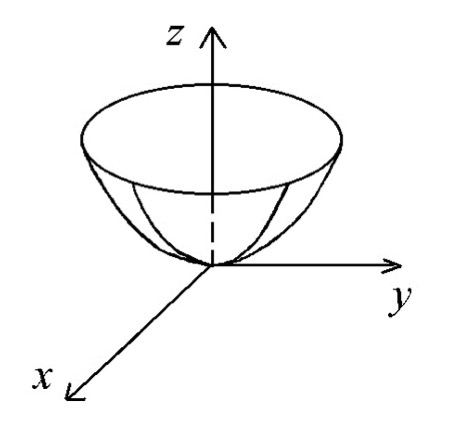
\includegraphics[width=.4\textwidth]{pic_1.jpg} & 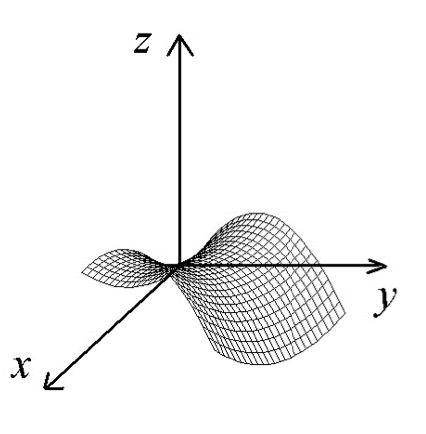
\includegraphics[width=.4\textwidth]{pic_2.jpg}\\
 Рисунок 1.1 - Полусфера & Риуснок 1.2 - Волна
\end{tabular}
\end{center}

Следовательно, для исследования локального экстремума нужны некоторые достаточные условия.

Предварительно вспомним алгебраические понятия. \cite{litlink1}


\begin{table}[H]
	\caption{График защиты курсовой работы}
	\begin{center}
		\begin{tabular*}{0.4\textwidth}{@{\extracolsep{\fill} } lcc}
			\toprule
			Дата & 12:00 & 17:00 \\
			\midrule
			20.12       & Долгов К.   & Калинин А.   \\
			23.12       & Суслопаров В.    & Волкович К.    \\
			25.12     & Сергеев А.   & Теребов М.   \\
			27.12      & Шестаков М.   & Драчева Е.    \\
			\bottomrule
		\end{tabular*}
		\label{tabular:tab_examp_1}
	\end{center}
\end{table}


\newpage
\section*{Заключение}

Цель работы достигнута: в ходе работы были оформлены  3 страницы математического текста с формулами и рисунками и таблица с профессиями согласно стандартам оформления. Данная работа помогла ознакомится с инструментами системы компьютерной верстки LaTeX.

\addcontentsline{toc}{section}{Заключение}